\begin{multicols}{2}

\begin{equation*}
    b)~\frac{1}{2} \sqrt{\frac{a^2 + b^2 + c^2}{2}}
\end{equation*}

\textsc{Указание. См. задачи 3, 4 в статье }\\
\indent \textbf{4. } Постройте тетраэдр до параллелипипеда вторым способом. 
Учетверенный квадрат длины каждого ребра параллелепипеда выразите по теореме косинусов через длины диагоналей
соответствующей грани и угол между ними (по дной грани на ребро).
Затем к граням параллелепипеда примените теорему о сумме квадратов длин диагоналилей параллелограмма
и сумме квадратов длин его сторон. Сложив все полученные равенства, получите требуемый результат. 

\vspace{0.5cm}
\begin{flushleft}
\textbf{К статье "Московский инженерно-физический институт"}\\
\vspace{0.2cm}
\textbf{Математика}\\
\vspace{0.2cm}
\textsc{Вариант 1}
\end{flushleft}

\indent 1. Обозначим скорости трех лыжников буквами (k=1, 2, 3) (\textit{м/мин}), а всю дистанцию через $S$ (м).
Третьему лыжнику после $m$ (мин) остается пройти расстояние ($S$=$m\nu_3$) (м).
По условию задачи это расстояние первый лыжник пройдет за $n$ минут, а второй - за $p$ минут.\\
\indent Учитывая эти условия и соотношения между скоростями, получим систему уравнений:
\begin{equation*}
 \begin{cases}
   \frac{S-m\nu_3}{\nu_1} = $n$,\\
   \frac{S-m\nu_3}{\nu_2} = \rho, \indent \indent (1) \\
   \nu_1 + \nu_2 = 2\nu_3.
 \end{cases}
\end{equation*}

Из системы (1) требуется найти отношения $\frac{S}{\nu_n}$
(k=1, 2, 3). Исключив из первых двух уравнений системы $S$=$m\nu_3$, получа-\\
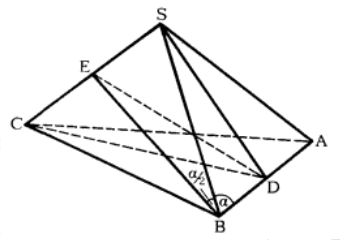
\includegraphics[width=0.45\textwidth]{scheme.png}


\begin{flushleft} ем систему уравнений для отношений $\frac{\nu_1}{\nu_3}$ и $\frac{\nu_2}{\nu_3}$ \end{flushleft}
\begin{equation*}
 \begin{cases}
   n \frac{\nu_1}{\nu_3} - \rho \frac{\nu_2}{\nu_3} = 0, \indent \indent (2) \\
   \frac{\nu_1}{\nu_3} + \frac{\nu_2}{\nu_3} = 2.
 \end{cases}
\end{equation*}


\indent Решение линейной алгебраической системы линейных уравнений с двумя неизвестными (2) имеет вид
\begin{equation*}
\frac{\nu_1}{\nu_3} = \frac{2\rho}{n + \rho},~
\frac{\nu_2}{\nu_3} = \frac{2n}{n + \rho}.
\end{equation*}

Теперь из первых двух уравнений системы (1) получим ответ:

\begin{center}
    $S/\nu_1$ = $(n + \frac{1}{2}m + \frac{mn}{2\rho})(\textit{мин})$, \\ \vspace{0.15cm}
    $S/\nu_2$ = $(\rho + \frac{1}{2}m + \frac{mn}{2n})(\textit{мин})$, \\ \vspace{0.15cm}
    $S/\nu_3$ = $(n + m + \frac{2n\rho}{n +\rho})(\textit{мин})$.\\
\end{center}

\indent 2. Из равенства плоских углов при вершинах А и В (см. рис. 1) следует,
что треугольники $ACB$ и $ACB$ - равные равнобедренные, поэтому $BC$ = $CA$ = $BS$ = $SA$
и $\alpha$ < $\frac{\pi}{2}$. Соединим середину $D$ отрезка $АВ$ с вершинами $С$ и $S$.
Плоскость $CDS$ перпендикулярная ребру $АВ$, так как медианы $CD$ и $SD$ равнобедренных треугольников
$ACB$ и $ACB$ одновременно являются высотам и этих треугольников. Объем $V$ пирамиды $SABC$ равен
сумме объемов пирамид $BDSC$ и $ADSC$,\\
\begin{equation*}
\indent V = \frac{1}{3} BD \cdot Q + \frac{1}{3} AD \cdot Q = \frac{1}{3} \frac{a}{3} \cdot Q, \indent (1)\\
\end{equation*}

где $Q$ - площадь треугольника $CDS$,
$BD$ = $DA$ = $\frac{1}{2}a$ (по построению). Таким образом, для нахождения объема пирамиды
достаточно вычислить площадь треугольника $CDS$.\\
\indent Треугольник $CDE$ - равнобедренный, так как $CD$ = $SD$ (это следует из равенстввапрямоугольных
треугольников $CDB$ и $SDB$, $DB$ … общая сторона, $\angle SBD$ = $\angle CBD$ = $\alpha$.
Проведем $DE \bot CS$ ($CE$ = $ES$ по свойству высоты равнобедренного треугольника). Следовательно,
\begin{equation*}
    Q = \frac{1}{2} CS \cdot DE = CE \cdot DE . \indent (2)
\end{equation*}
Величины отрезков $CE$ и $DE$ легко находятся из прямоугольных треугольников $ВЕС$


\end{multicols}
\newpage
Табличка рандомной функции, ибо в этом выпуске их нема

\begin{tabular}{l|l}
    \hline
    X & Y\\
    \hline\hline
    -10	& 999993085000 \\
    -9	& 282425451165 \\
    -8	& 68717208064 \\
    -7	& 13840122373 \\
    -6	& 2176242552 \\
    -5	& 243923125 \\
    -4	& 16705600 \\
    -3	& 514269 \\
    -2	& 1768 \\
    -1	& -83 \\
    0	& 0 \\
    1	& 85 \\
    2	& 6424 \\
    3	& 548613 \\
    4	& 16848832 \\
    5	& 244358125 \\
    6	& 2177322120 \\
    7	& 13842452029 \\
    8	& 68721745408 \\
    9	& 282433621797 \\
    10	& 1000006915000
\end{tabular}

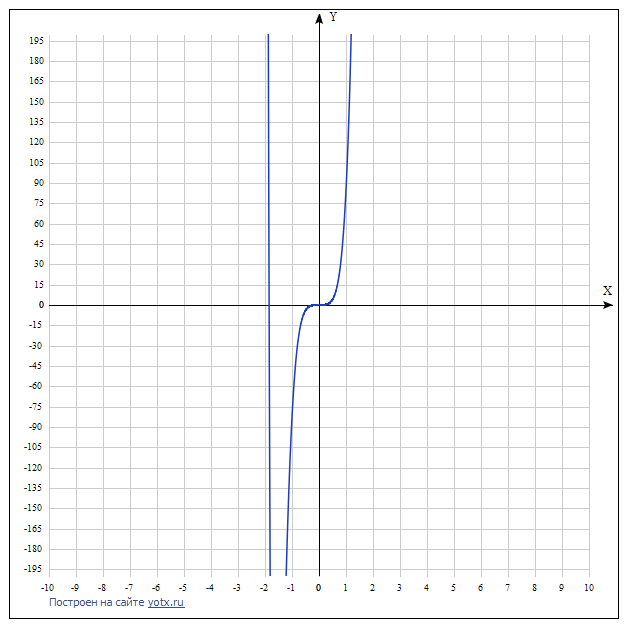
\includegraphics[width=0.7\textwidth]{func_img.png}


\newpage
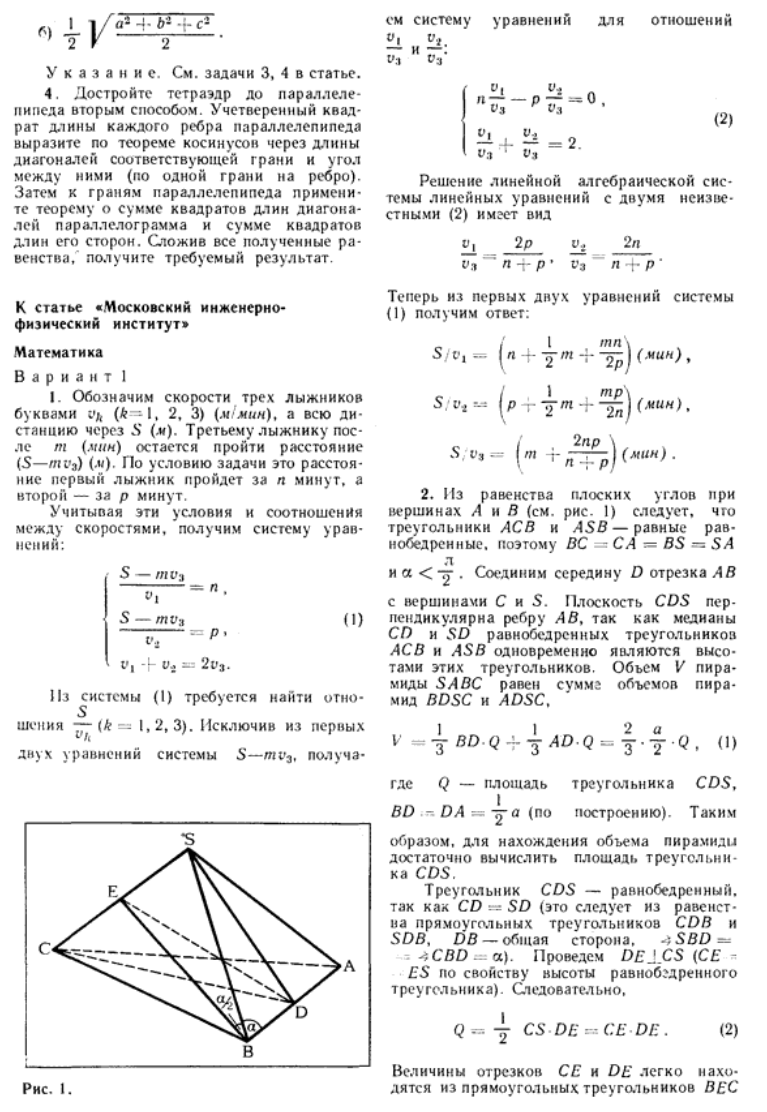
\includegraphics[width=0.95\textwidth]{orig.png}

\newpage
Исходники:\\
\url{https://github.com/ArsenyVekshin/ITMO/tree/master/Inf/lab6} \\